%------------------------------------------------------------------------------
% physor2014_template.tex - template to write a contribution for the PHYSOR 
% 2014 conference
% v1.0 20130422 Wilfred van Rooijen, University of Fukui
%------------------------------------------------------------------------------
% Usage: this template file should be used ONLY with pdfLaTeX. Users who
%        normally use LaTeX need to convert their figures from (E)PS to PDF.
%        See the end of this file for several tips & tricks. Place this 
%        template file and the file physor2014.sty in the same working
%        directory. If you use bibtex, put physor.bst and physor2014.bib also
%        in the working directory. If you have your own BiBTeX database file,
%        make a copy or link in your working directory and replace 
%        \bibliography{physor2014} with \bibliography{your_bib_file}.
%
% NOTE: when running the PHYSOR2014 style file, you may get warnings regarding
%       the versions of several of the style files used in the PHYSOR2014 tem-
%       plate. These are indications that it is time to update you latex in-
%       stallation, but even if you use the older versions, the PHYSOR2014 tem-
%       plate should work correctly. 
%------------------------------------------------------------------------------
\documentclass[12pt]{article}
%
% NOTE: use \documentclass[12pt,draft]{article} for your initial work. This 
%       will give you the "draft" mode:
%       - a black marker is printed for each "overfull hbox"
%       - figures are not included (only the BoundingBox is indicated)
%       - hyperref is switched off
%
% When your manuscript has "overfull" or "underfull" boxes (see latex output)
% then that means that LaTeX cannot perform a proper line breaking. You can try
% to solve the problem by:
% - adding hyphenation locations in long words: hy\-phe\-na\-tion
% - rewrite the sentence
% - adding space, e.g. "Author \cite{foo}" instead of "Author\cite{foo}"
% Try to get rid of all the underfull and overfull boxes (but sometimes a small
% amount of overfull cannot be avoided). 
%
\usepackage{physor2014}
%
% The basic style file loads a minimum of style files. If you need special 
% styles, simply include them here. For example, you may be interested in the
% following packages.
%
% For anything that involves mathematics, equations, etc
\usepackage{amsmath}
%
% To include figures in your paper. Note the following: manuscripts must be
% prepared in PDF. To do this, use pdflatex to produce PDF directly. pdflatex
% can include figures in the following formats: PDF, JPG, and PNG. For bitmap-
% ped images (photos etc), JPG is the preferred format, because JPG images can 
% be compressed very well in PDF, giving very small PDF files. For graphs and 
% schematics, vector images should be used; these can be either PostScript or
% PDF. If you have your figures as (e)ps, then see the notes at the end of this
% file for how to convert (e)ps to pdf.
%
% Making PDF images with Excel: see
% http://office.microsoft.com/en-us/word-help/convert-a-document-to-pdf-HA102850064.aspx?CTT=1
% To make very pretty drawings with LaTeX, check out PGF/TikZ
%
\usepackage{graphicx}
%
% If you use a table, check out this package. It creates tables with a little
% bit more space around the table entries. The result is a table that is easier
% to read, especially if you have mathematical super/subscripts in your work.
% Also check the manual of the package booktabs because it has some good tips 
% on how to make beautiful and informative tables.
\usepackage{booktabs}
%
% The following package takes care of setting SI units. Simply type 
% \degreeCelsius instead of $^\circ$ C. Also takes care of exponents and powers 
% of ten, as well as lining out numbers on the decimal point if required
% \usepackage{siunitx}
%------------------------------------------------------------------------------
%\usepackage{tikz}
\usepackage{amsfonts}
%\usepackage[usenames,dvipsnames]{xcolor}
%\usepackage{tikz}
%\usetikzlibrary{shapes,arrows,calc,3d,chains,fit,decorations}
\usepackage{subcaption}

\newcommand{\bs}{\boldsymbol}

\newcommand{\eqt}[1]{Eq.~(\ref{#1})} % equation
\newcommand{\fig}[1]{Fig.~\ref{#1}} % figure
\newcommand{\tbl}[1]{Table~\ref{#1}} % table
\newcommand{\sect}[1]{Section~\ref{#1}} % section
\newcommand{\subsect}[1]{Subsection~\ref{#1}} % subsection
\newcommand{\app}[1]{Appendix~\ref{#1}} % appendix

\newcommand{\ie}{i.e.,\@\xspace}
\newcommand{\eg}{e.g.,\@\xspace}
\newcommand{\psc}[1]{{\sc {#1}}}
\newcommand{\rs}{\psc{R7}\xspace}
\renewcommand{\div}{\nabla \cdot}
\newcommand{\grad}{\nabla}

%------------------------------------------------------------------------------
% Define title. Use all CAPITALS.
%------------------------------------------------------------------------------
\title{Extension of the Entropy Viscosity Method to Flows with Friction Forces and Source Terms}
%
% ...and authors
%
\author{ 
  \textbf{Marco Delchini, Jean C. Ragusa} \\
  Department of Nuclear Engineering \\
  Texas A\&M University, College Station, USA\\
  \href{mailto:marco.delchini@gmail.com}{marco.delchini@gmail.com}, 
  \href{mailto:jean.ragusa@tamu.edu}{jean.ragusa@tamu.edu}\\
   % Put an extra empty line for different affiliations 
  \textbf{Ray A. Berry} \\
  Idaho National Laboratory\\
  Idaho Falls, ID, USA\\
  \href{mailto:ray.berry@inl.gov}{ray.berry@inl.gov}
}

%------------------------------------------------------------------------------
% The \shortauthor is printed on top of the even pages, and the \shorttitle
% is printed on top of the odd pages.
% Suggested format:
% - One author             : A. Author
% - Two authors            : A. Author \& B. Author
% - Three authors          : A. Author, B. Author \& C. Author
% - More than three authors: A. Author~et~al.
% If the title of your manuscript is very long, then make a short title such
% that it fits on one in the header of the odd pages.
%------------------------------------------------------------------------------
\renewcommand{\shortauthor}      % Author's names here
           {Delchini, Ragusa, Berry}  
\renewcommand{\shorttitle}       % Short title here
           {Entropy Viscosity Method with Friction and Source Terms}  

%------------------------------------------------------------------------------
% Setup PDF info. This sets several values which are listed as the "properties"
% of the PDF file.
%------------------------------------------------------------------------------
\hypersetup{
  pdftitle=\shorttitle,
  pdfauthor=\shortauthor
}

%------------------------------------------------------------------------------
% Begin document
% You can use \doublespacing for your personal draft. This option will increase
% the line spacing, making it easier to add written comments etc. Be sure to
% switch it off when you make the final version!
% The command \linenumbers switches on line numbers, which are practical when
% reviewing a manuscript. Switch off line numbers when you make your final
% version. 
%------------------------------------------------------------------------------
\begin{document}

%\doublespacing

%\linenumbers

%------------------------------------------------------------------------------
% Make the titlepage and set the pagestyle to fancy throughout
%------------------------------------------------------------------------------
\maketitle

\begin{abstract}
In this paper, we extend the entropy viscosity method \cite{valentin, jlg1, jlg2} to $1$-D Euler equations with source terms present. 
The entropy viscosity method has been successfully applied to hyperbolic equations such as Burgers equation and the Euler
equation system. This method consists in adding dissipative terms to the governing equations so as to ensure the entropy minimum principle. The dissipative terms contain a viscosity coefficient (function) that locally modulates the amount of dissipation.
This viscosity coefficient is based on the entropy production that occurs in the wiggles, discontinuities, and shocks of hyperbolic equation systems.
By adding source terms to the Euler equations (friction and gravity forces to the momentum equation and heat sources/sinks in the energy equation), the entropy viscosity method must be modified to account for the entropy production due to these additional terms. Tests are run for a 1D channel, using pressurized water reactor (PWR) conditions, with the RELAP-7 code \cite{relap7} based on the MOOSE framework \cite{Moose}. The equations are discretized with a continuous Galerkin finite element method (FEM) using linear polynomials along with a second-order, implicit temporal scheme (BDF2).
\end{abstract}

\keywords{entropy-based viscosity scheme, Euler equations with source terms, viscous regularization, low Mach flow}

%------------------------------------------------------------------------------
%
%------------------------------------------------------------------------------
\section{Introduction}
\label{sect::intro}

Hyperbolic systems of equations are challenging to solve numerically, due to the presence of shocks. Godunov upwind schemes are overly
dissipative and only first-order accurate, while higher order methods need flux  limiters to prevent unphysical oscillations. Recently,
a new technique to stabilize hyperbolic equations has been introduced \cite{valentin, jlg1, jlg2} . 
It requires the addition of artificial dissipation terms to the equations, while ensuring that the entropy minimum principle remains satisfied. 
This technique, called the \emph{entropy viscosity method}, is independent of the spatial discretization and thus can be used with a standard 
Galerkin finite element method (FEM).  We have developed the fluid solver used here within Idaho National Laboratory's RELAP-7 code \cite{relap7} (which uses the MOOSE framework \cite{Moose}), with the goal of applying the entropy viscosity method to fluid flow problems for nuclear reactor applications. Therefore, it is crucial to stress the capabilities of the method beyond standard Euler equations. Specifically, we analyze the implication of adding wall friction, gravity, and heat sources/sinks to the conservation equations.
A 1D channel, with conditions representative of those in a PWR, are used in our numerical tests. This test case also presents the challenge
of employing a conservative formulation in the low-Mach limit, an asymptotic region not yet tested with the entropy viscosity method. In Section~\ref{sec:section1}, we first recall
the fundamentals of the entropy viscosity method.  Its extension to Euler equations with friction forces, gravity forces, and heat sources/sinks is presented in Section~\ref{sec:ext}. Numerical results are provided in Section~\ref{sec:results} using this entropy viscosity method, along with those obtained using the SUPG stabilization method  \cite{SUPG} for comparison purposes.


%------------------------------------------------------------------------------
%
%------------------------------------------------------------------------------
\section{Entropy viscosity method: a review for single-phase Euler equations}
\label{sec:section1}

The entropy-based viscosity method \cite{valentin, jlg1, jlg2} is recalled for the multi-dimensional Euler equations \cite{Toro}, with no source or friction terms added at this stage. The entropy viscosity method consists of adding appropriate dissipative terms, with a viscosity coefficient modulated by the entropy production. The scheme detects shocks (entropy production is large in shocks) and mitigates the unphysical oscillatory behavior usually associated with high-order schemes for conservation equations. The derivation of the artificial dissipative terms to be added to the Euler equations can be found in \cite{jlg}, and are recalled below, in \eqt{eq:euler_visc}. Formally, solutions to Euler equations should satisfy the entropy minimum principle, i.e., 
\begin{equation}
\partial _t s + u \cdot \grad s \ge 0 
\end{equation}
where $s$ is an entropy function. The viscous regularization of \cite{jlg} reproduces this property such that
\begin{equation}
\rho \big( \partial _t s + u \cdot \grad s \big) + \text{conservative terms} \ge 0 .
\end{equation}
The viscous regularization yields conservative terms of the form $-\div K \grad s$ and a right-hand-side contribution that is positive. The Euler equation with viscous regularization are:
\begin{equation}
\label{eq:euler_visc}
\left\{ 
\begin{array}{lll}
\partial_t \left( \rho \right) + \nabla \cdot \left( \rho \vec{u} \right) = \nabla \cdot \left( \kappa \nabla \rho \right) \\
\partial_t \left( \rho \vec{u} \right) + \nabla \cdot \left( \rho \vec{u} \otimes \vec{u} + P I \right) = \nabla \left( \mu \rho \nabla \vec{u}  + \kappa \vec{u} \otimes \nabla \rho \right)  \\
\partial_t \left( \rho E \right) + \nabla \cdot \left[ \vec{u} \left( \rho E + P \right) \right] = \nabla \cdot \left( \kappa \nabla \left( \rho e \right) + \frac{1}{2}|| \vec{u} ||^2 \kappa \nabla \rho +  \rho \vec{u} \mu \nabla \vec{u}  \right) \\
P = P\left( \rho, e \right)
\end{array}
\right.
\end{equation}
where $\kappa$ and $\mu$ are local positive viscosity coefficients.

We have assumed the existence of a specific entropy function $s$, dependent upon the internal energy $e$ and density $\rho$.  We further require the convexity of $-s$ with respect to $e$ and $\frac{1}{\rho}$, along with the partial derivatives of $s$ satisfying: $P \partial_e s + \rho^2 \partial_{\rho} s = 0$.
%obtained is valid for any equation of state as long as the opposite of the physical entropy function is convex.

In the current version of the method, the local viscosity coefficients $\kappa$ and $\mu$ are set equal, so that the above viscous regularization (\eqt{eq:euler_visc}) is equivalent to the parabolic regularization \cite{Parabolic}. The current definition also includes a first-order viscosity coefficient denoted with the subscript $max$, and a high-order viscosity coefficient denoted with the subscript $e$. The \emph{first-order viscosity coefficients} $\mu_{max}$ and $\kappa_{max}$ are proportional to the largest local eigenvalue $|| \vec{u} || + c $ : 
\begin{equation}
\label{eq:equation15}
\mu_{max}(\vec{r}, t) = \kappa_{max}(\vec{r}, t) = \frac{h}{2} \left( || \vec{u} || + c \right),
\end{equation}
where $h$ is the grid size.  The first-order viscosity coefficients are equivalent to a first-order upwind-scheme, which is known to to be monotone but overly-dissipative \cite{Toro}.
The \emph{higher-order viscosity coefficients} $\kappa_e$ and $\mu_e$ are set proportional to the entropy production, which is evaluated by computing the local entropy residual $D_e$, and to the jump $J$ of the entropy flux, which enables the detections of discontinuities others than shocks:
\begin{equation}
\label{eq:ent_visc_coeff}
\mu_e(\vec{r},t) = \kappa_e(\vec{r},t) = h^2 \frac{\max\left( | D_e(\vec{r},t) |, J \right)}{|| s - \bar{s} ||_{max}} \text{ with } D_e(\vec{r}, t) = \partial_t s + \vec{u} \cdot \nabla s
\end{equation}
where $|| \cdot ||_{max}$ and $(\bar{\cdot})$ denote the infinite norm operator and the average operator over the entire computational domain, respectively. The definition of the jump $J$ is discretization-dependent and examples of such can be found in \cite{valentin} for DGFEM. The normalization of the denominator $|| s - \bar{s} ||_{max}$ is used for dimensionality purposes.
% and should not be of the same order as $h$, on penalty of loosing the high-order accuracy. Currently, there are no theoretical justification for choosing the denominator. \\

The definitions of the viscosity coefficients $\mu$ and $\kappa$ are functions of the first- and higher-order viscosity coefficients as follows:
\begin{equation}
\label{eq:mu}
\mu(\vec{r},t) = \min\left( \mu_e(\vec{r},t), \mu_{max}(\vec{r},t) \right) \text{ and } \kappa(\vec{r},t) = \min\left( \kappa_e(\vec{r},t), \kappa_{max}(\vec{r},t) \right).
\end{equation}
In shock regions, the higher-order viscosity coefficients exhibit large values because of the entropy production, and saturate to the overly-dissipative first-order viscosity, and will smooth out oscillations. Everywhere else, the entropy production is negligible and the viscosity coefficients $\mu$ and $\kappa$ are of order $h^2$, and small.
Using these definitions of the entropy-based viscosity method, high-order accuracy was demonstrated and good results were obtained with 1-D Sod shock tubes and various 2-D tests \cite{valentin, jlg1, jlg2}.

The current definition of the viscosity coefficients requires an analytical expression of the entropy function $s$ which can be difficult to obtain when dealing with complex equations of states; and, does not seem to be adapted to low Mach flows that are known to be isentropic. Furthermore, the entropy residual $D_e(\vec{r},t)$ and the denominator $|| s - \bar{s} ||_{max}$ will both tend to zero, leading to an undetermined form. This motivates us to modified the expression for the entropy residual (using the chain rule) so as to make it a function of pressure and  density: 
\begin{equation}
\label{eq:new_ent_res}
D_e(\vec{r},t) = \partial_t s + \vec{u} \cdot \nabla s = \frac{s_e}{P_e} \underbrace{\left( \frac{d P}{dt} - c^2 \frac{d \rho}{dt} \right)}_{\tilde{D}_e(\vec{r},t)},
\end{equation}
where $\frac{d \cdot}{dt}$ denotes the material or total derivative, and $P_e$ is the partial derivative of the pressure $P$ with respect to the internal energy $e$. Because $D_e(\vec{r},t)$ and $\tilde{D}_e(\vec{r},t)$ are proportional to each other, the definition of the viscosity coefficients $\mu$ and $\kappa$ can rely on $\tilde{D}_e(\vec{r},t)$ without affecting the heart of the entropy viscosity method as follows: 
\begin{equation}
\label{eq:ent_visc_coeff2}
\mu_e(\vec{r},t) = \kappa_e(\vec{r},t) = h^2 \frac{\max\left( | \tilde{D}_e(\vec{r},t) |, J \right)}{(1-M) \rho c^2 + M \rho |\vec{u}|^2} \,.
\end{equation}
The changed denominator, as shown in \eqt{eq:ent_visc_coeff2}, is of the same dimension as the pressure. As a function of the Mach number $M$, the speed of sound $c$, the density $\rho$, and the norm of the velocity vector $|\vec{u}|^2$, it ensures consistency of the viscosity coefficients when dealing with low Mach flows. Here the jump $J$,  is chosen to be proportional to the jump of the pressure and density gradients at the interfaces:
\begin{equation}
\label{eq:equation23}
J_{i+1/2} = |\vec{u}|_{i+1/2} \max \left( [[ \nabla P \cdot \vec{n} ]]_{i+1/2}, c^2 [[ \nabla \rho \cdot \vec{n} ]]_{i+1/2} \right) \text{ with } [[ \cdot ]] = |(\nabla \cdot)_i -  (\nabla \cdot)_{i+1}| \cdot \vec{n},
\end{equation}
where $i+1/2$ denotes the interface between cells $i$ and $i+1$, and $\vec{n}$ is its outward normal.
The definition of the viscosity coefficients $\mu$ and $\kappa$ remain unchanged, as well as the dissipative terms.

%------------------------------------------------------------------------------
%
%------------------------------------------------------------------------------
\section{Extension of the entropy viscosity method to include friction, gravity, and sink/source terms}
\label{sec:ext}

Next, we show that the entropy viscosity method can be modified to retain its validity when adding source terms to the $1$-D Euler equations. Gravity and the wall friction forces are added in the momentum equation and a wall-heat source is supplied in the energy equation, omitting the artificial dissipative terms:
\begin{equation}
\label{eq:equation19}
\left\{
\begin{array}{lll}
\partial_t \rho + \nabla_x  \cdot \left( \rho u \right) = 0 \\
\partial_t \left( \rho u \right) + \nabla_x \cdot \left( \rho u^2 + P \right) =  - \frac{A}{2 D_h} \rho f |u| u - \rho g \\
\partial_t \left( \rho E \right) + \nabla_x \cdot \left[ u  \left( \rho E + P \right) \right] = a_w h_w \left( T - T_w \right) - \rho g u
\end{array}
\right.
\end{equation}
where $f$ is a positive friction factor, $g$ is the gravity constant, and $D_h$ is the hydraulic diameter given by $D_h = 4A/p$ (A and p being the channel cross-sectional area and wetted perimeter, respectively). The variables $a_w$, $T_w$ and $h_w$ denote the heated surface, the wall temperature, and the wall heat transfer coefficient, respectively.
Wall friction does not affect the total energy equation because  the velocity at the wall is zero, thus no power is induced by the wall friction forces. 

Because the entropy residual method relies on the sign of the entropy residual, we need to understand how source terms affect the entropy residual. To accomplish this, we repeat the derivation of the entropy residual, with source terms included. Following the same steps detailed in \cite{jlg}, the entropy residual is obtained (note, gravity dependent terms cancel out):
\begin{equation}
\label{eq:equation20}
\rho \frac{ds}{dt} = \rho \frac{s_e}{P_e}\left( \frac{dP}{dt} - c^2 \frac{d \rho}{dt} \right) = s_e \left( a_w h_w (T - T_w) + \frac{\rho}{2 D_h} f |u| u^2 \right) .
\end{equation}
To prove the entropy minimum principle, the sign of the right-hand side of \eqt{eq:equation20} must be examined. Because $s_e$ is positive by definition \cite{jlg}, the sign of the right hand side will depend upon the terms inside the brackets. We observe that the friction term is always positive and, therefore, will not affect the sign of the entropy residual. However, the sign of the wall heat source term can be either positive or negative, depending upon whether or not $T$ is larger or smaller than $T_w$, and thus needs to be included in the definition of the entropy viscosity coefficients $\mu_e$ and $\kappa_e$. In order to account for the entropy production due to heating/cooling we use
\begin{equation}
\label{eq:equation21}
\mu_e(\vec{r},t) = \kappa_e(\vec{r},t) = h^2 \frac{\max\left( | \tilde{D}_e(\vec{r},t) |, | D_w(\vec{r},t) |, J \right)}{(1-M) \rho c^2 + M \rho |\vec{u}|^2} \, \text{ with } D_w(\vec{r},t) = a_w h_w (T - T_w).
\end{equation}
The definitions of the first order viscosity coefficients given in \eqt{eq:equation15} remain unchanged, as well as those for the viscosity coefficients $\mu$ and $\kappa$ (\eqt{eq:mu}).

%------------------------------------------------------------------------------
%
%------------------------------------------------------------------------------
\section{Numerical results for a Pressurized Nuclear Reactor PWR}
\label{sec:results}

Numerical tests are performed for a $1$-D pipe of cross-section $A = 7.854\, 10^{-5}$ $m^2$ and length $L=3.865$ $m$ with the following parameters: the heat transfer coefficient $h_w$ is set to a constant $5.33\, 10^4$ $W/(m^2.K)$, the heated perimeter $a_w$ is computed from $A$ and $L$ and set to $0.0298$ $m$, and the friction factor is constant and equal to $0.01$. The wall temperature $T_w$ is given spatial dependence and computed using the model available in RELAP-7 for PWR \cite{Relap7PWR}. 
%the heat source is constant and set to $7.7E+4$ $W/m^3$. 
%\begin{equation}
%\label{eq:equation24}
%h_w(x,t) = h_{w,0}(1-e^{-t})\sin \left( \frac{\pi}{2L} x\right) \text{ with } h_{w,0} = 5.33 \cdot 10^4 W / m.
%\end{equation}
For boundary conditions, we impose, at the inlet, a mass inflow ($\rho u = 3359.62$ $kg/(m^2.s))$ and a specific enthalpy ($h = 1.28\,10^6$ $J/kg$) and employ a static pressure condition at the exit ($P_s = 155$ bar). The stiffened gas equation of state (SGEOS) is used \cite{SGEOS} with the following parameters: $P_{\infty} = 8.5 \cdot 10^8$ Pa, $q = -1151\, 10^3$ $J/kg$, $\gamma = 2.04$ and $C_v = 2069$ $J/(kg.K)$. The steady-state is reached at around $t=150\,s$ with a time step of $\Delta t = 0.5\,s$. Figures~\ref{fig:Pressure} through~\ref{fig:Viscosity} represent the results obtained using 20 mesh cells, using either the overly-dissipative first-order viscosity (FO), the higher-order entropy viscosity (EV), or the SUPG method to stabilize the numerical scheme. From these figures, it is clear that employing the first-order viscosity leads to erroneous answers, while the entropy-viscosity results are correct and look similar to those obtained with the SUPG method. Plots obtained using a finer spatial resolution ($100$ cells) are also shown in these figures.

\begin{figure}[h]
\centering
%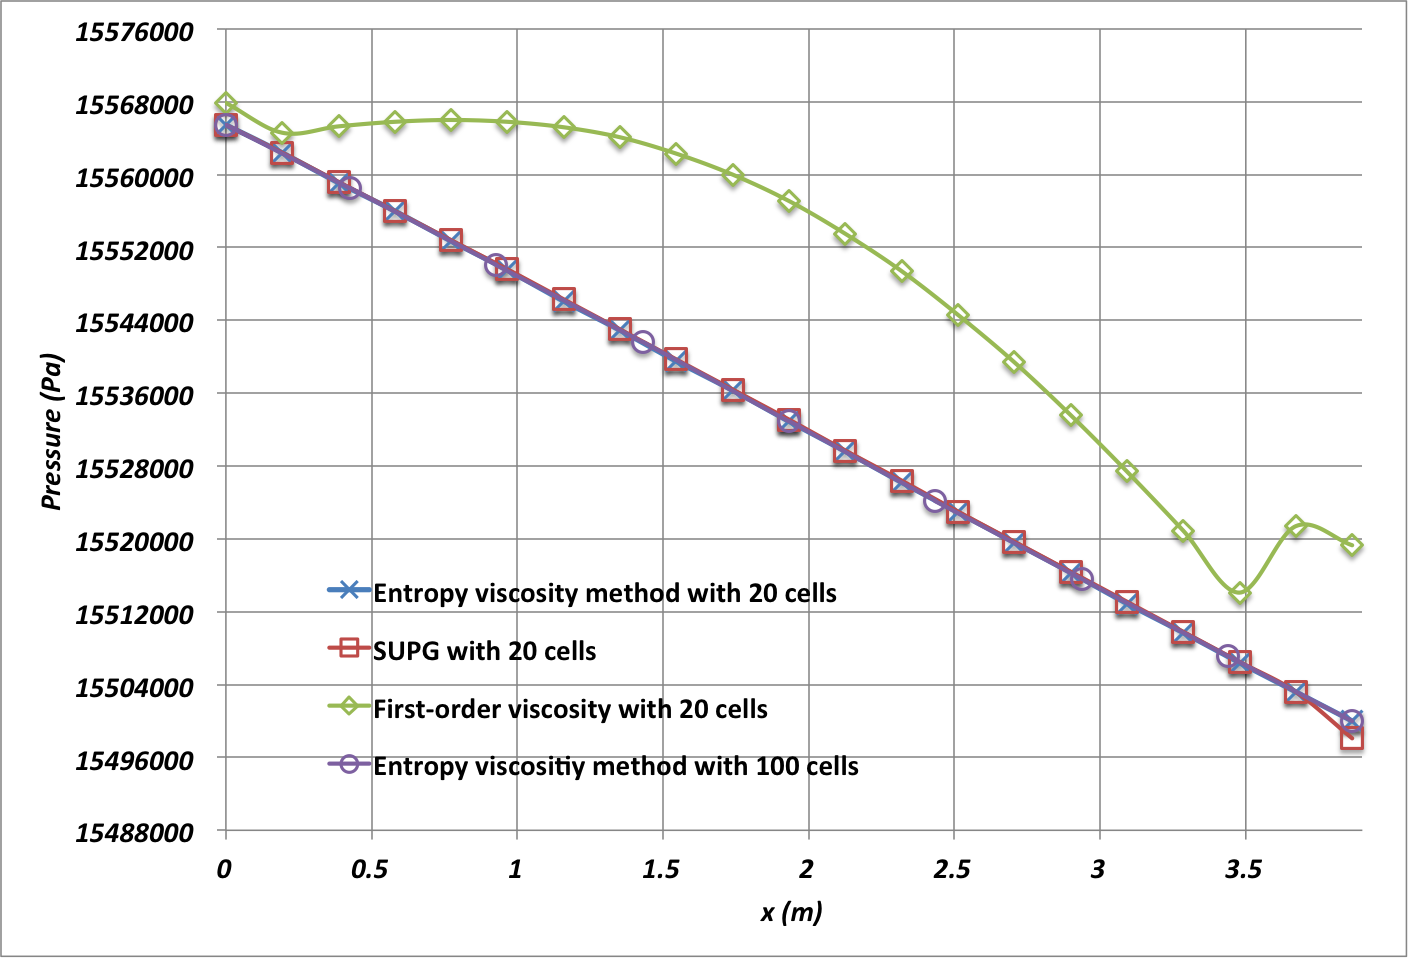
\includegraphics[scale=0.4]{plots/Pressure.png}
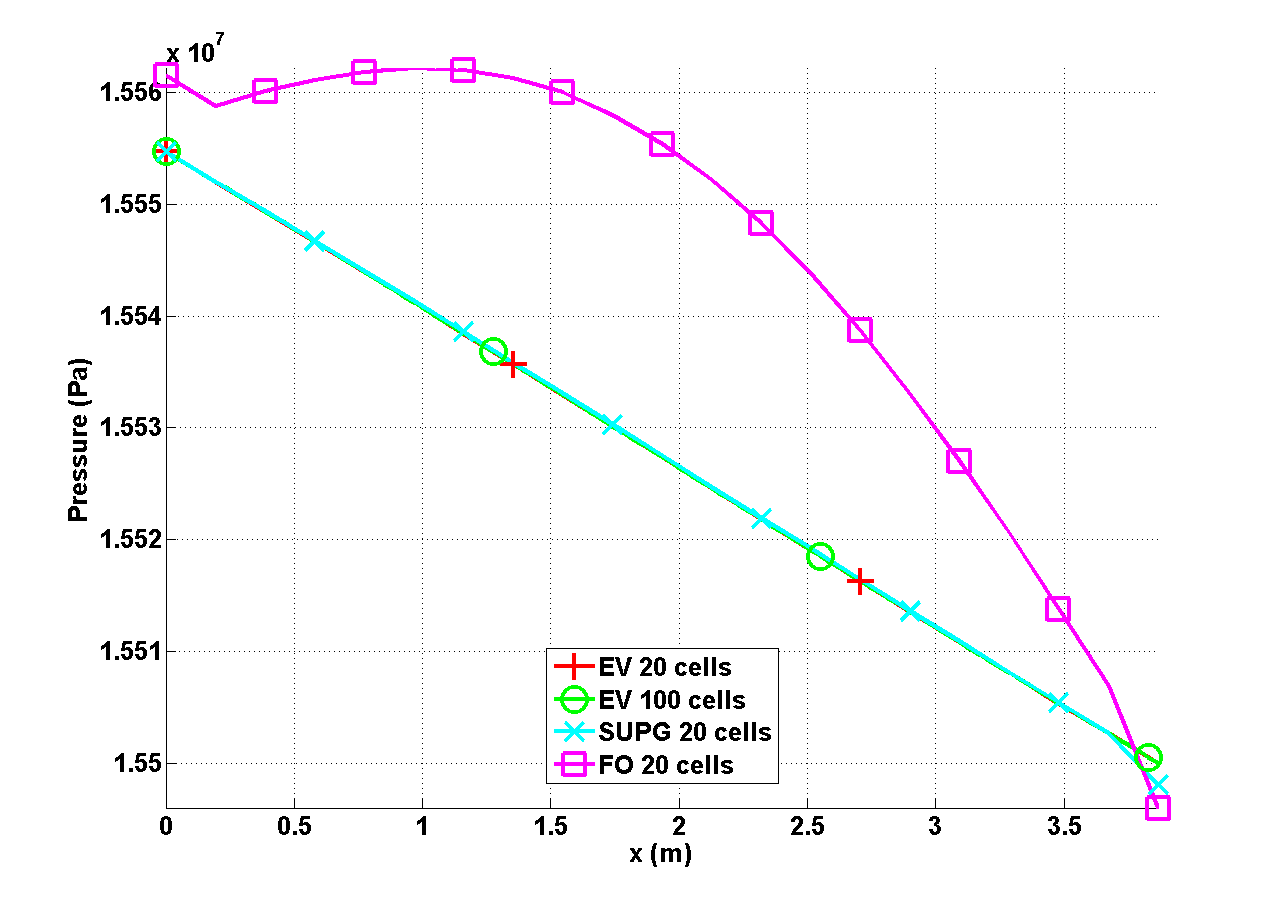
\includegraphics[scale=0.4]{plots/PWR_stt_pressure.png}
\caption{PWR test case: axial pressure profile}
\label{fig:Pressure}
\end{figure}
\begin{figure}[h]
\centering
%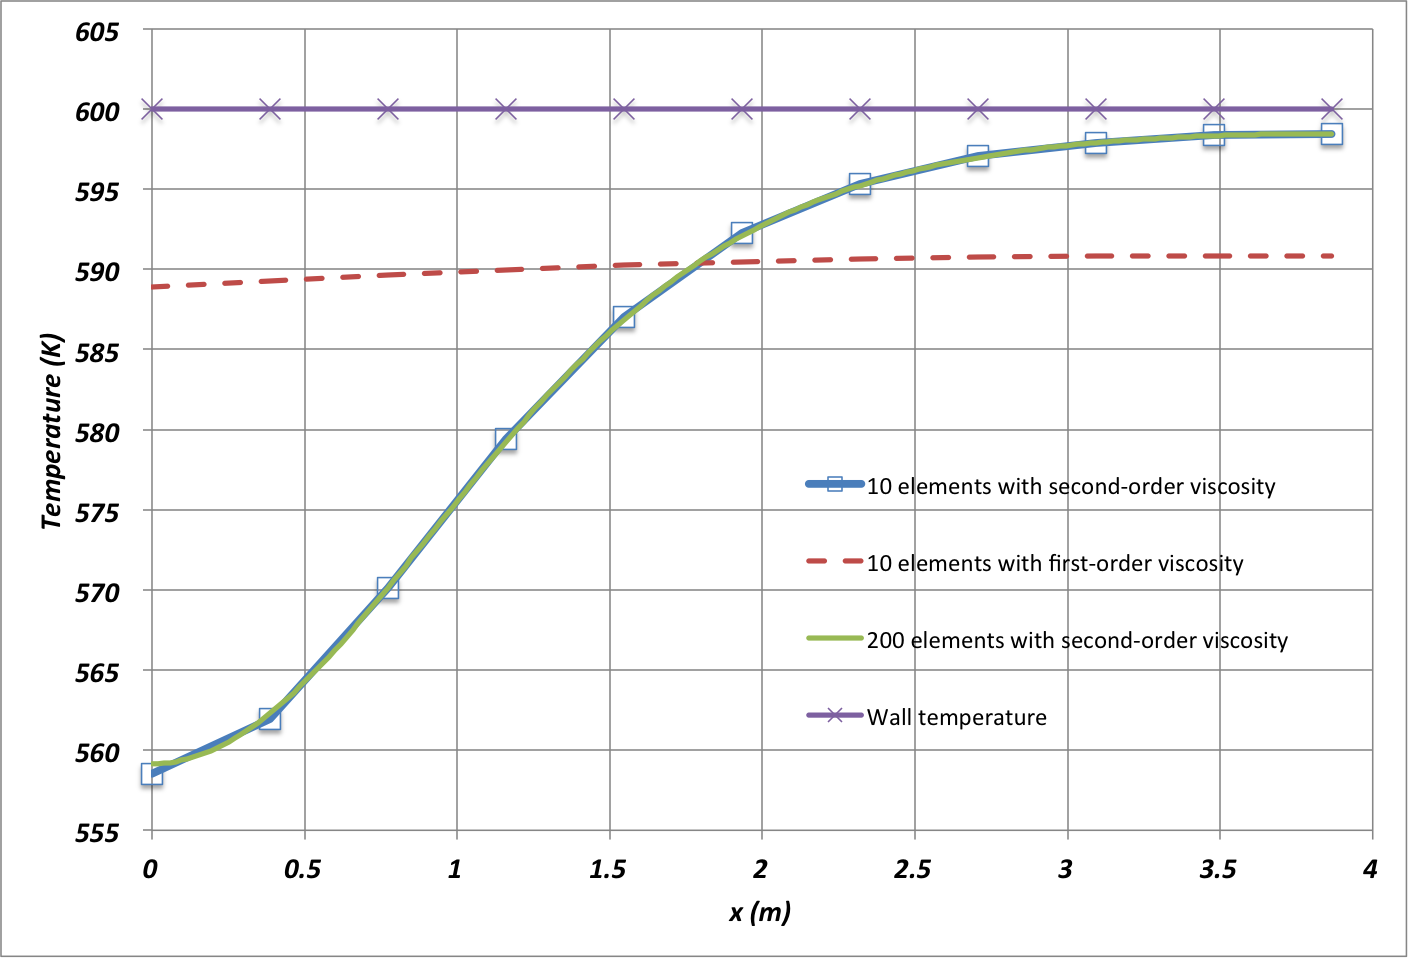
\includegraphics[scale=0.4]{plots/Temperature.png}
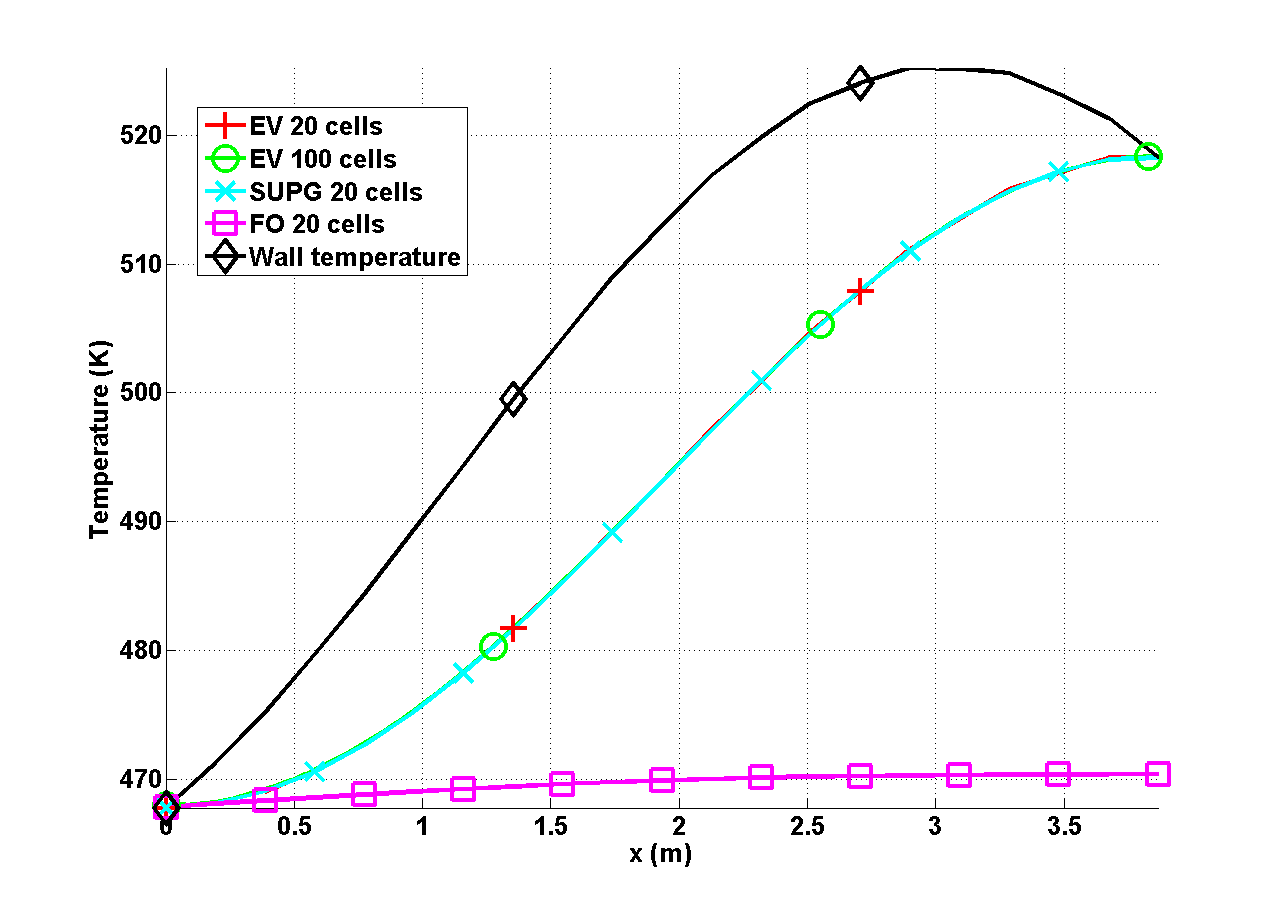
\includegraphics[scale=0.4]{plots/PWR_stt_temperature.png}
\caption{PWR test case: axial temperature profile}
\label{fig:Temperature}
\end{figure}
\begin{figure}[h]
\centering
%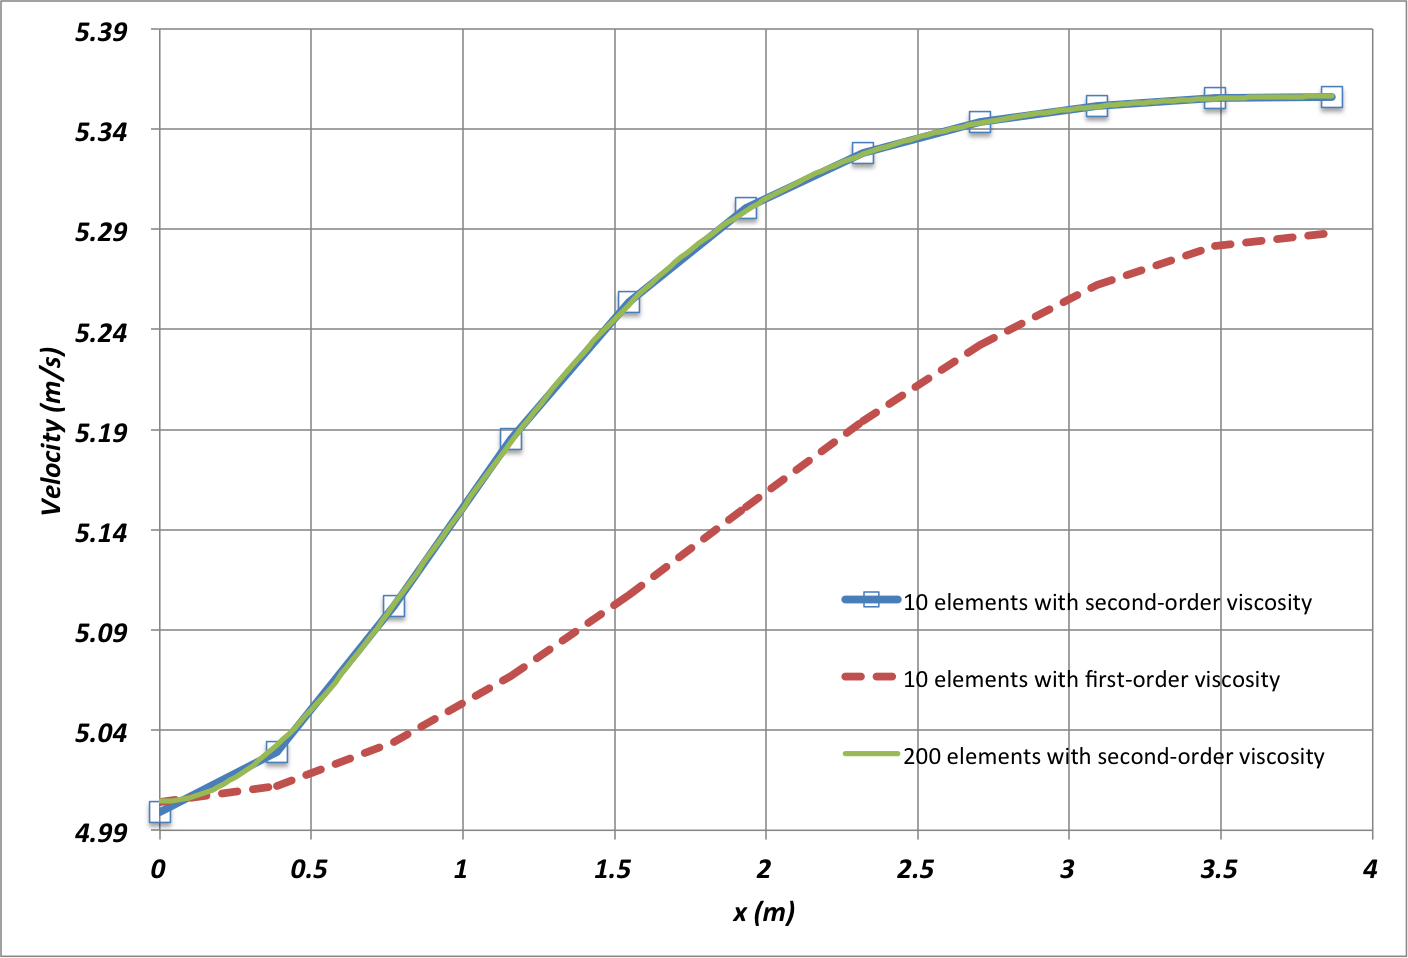
\includegraphics[scale=0.4]{plots/Velocity.png}
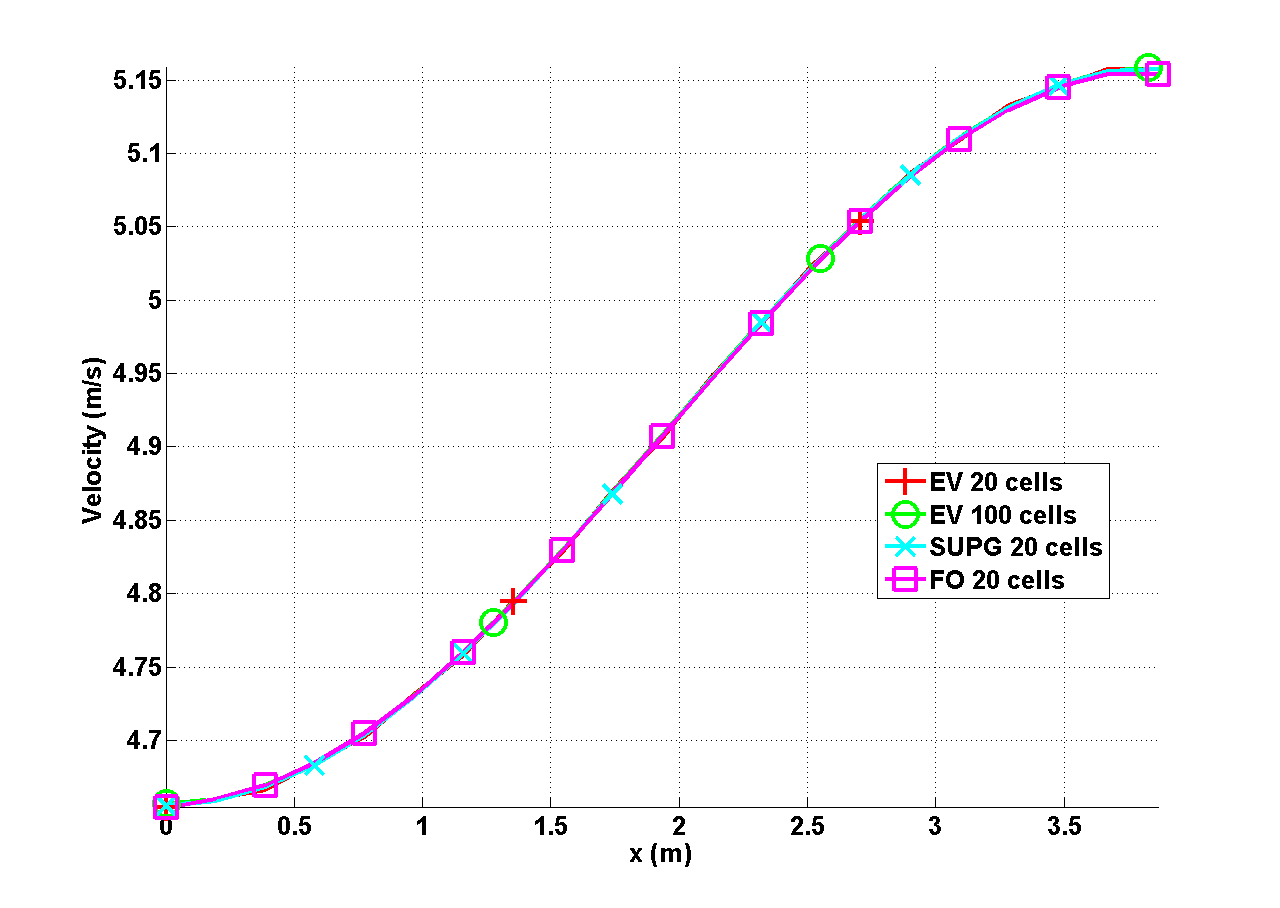
\includegraphics[scale=0.4]{plots/PWR_stt_velocity.png}
\caption{PWR test case: axial velocity profile}
\label{fig:Velocity}
\end{figure}
\begin{figure}[h]
\centering
%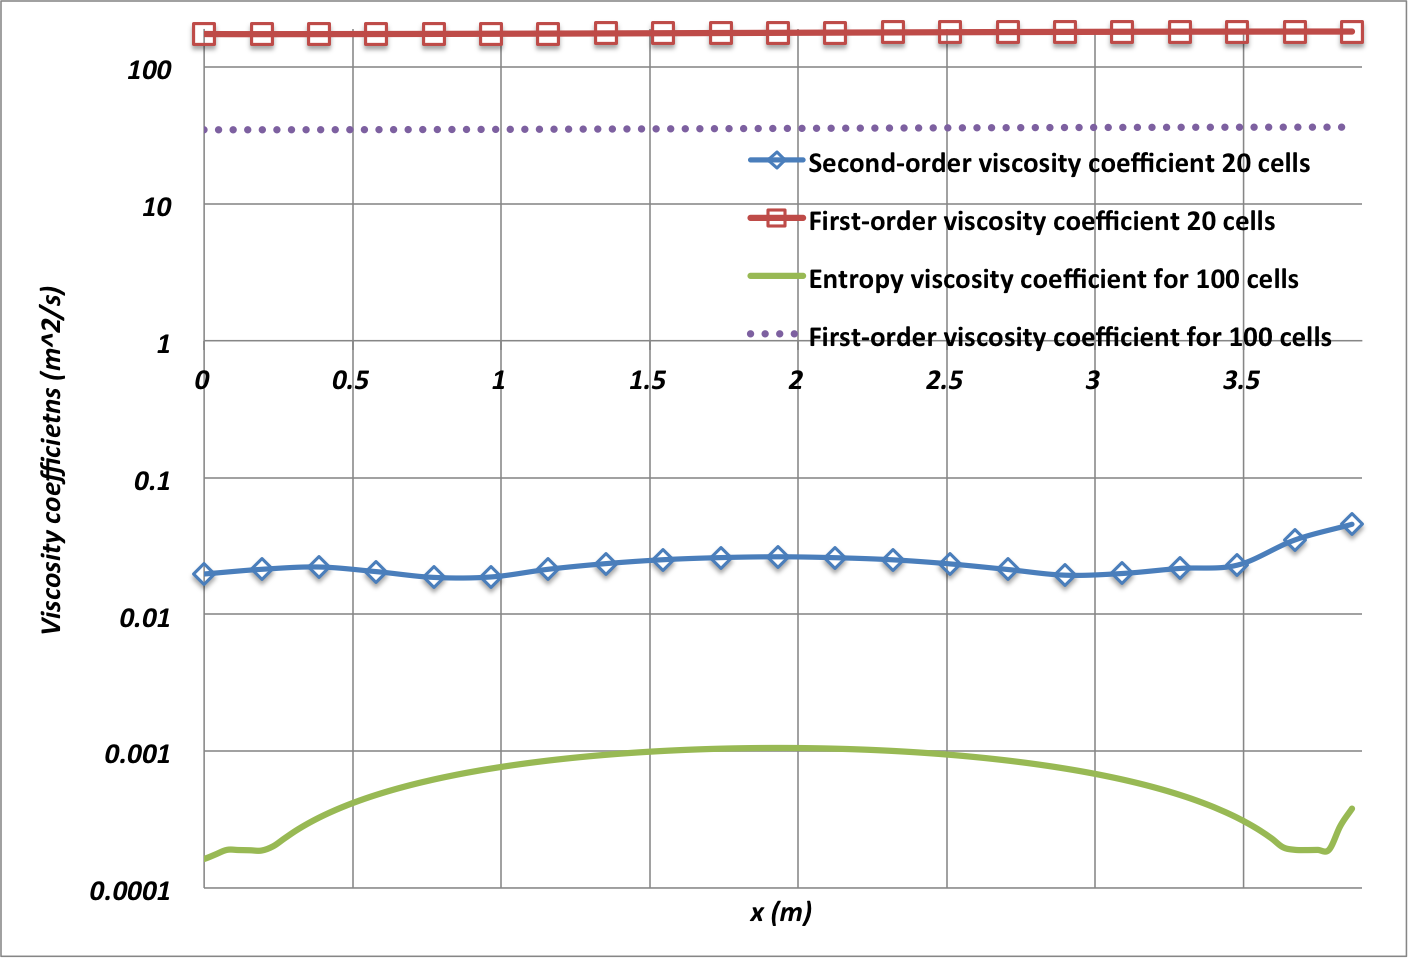
\includegraphics[scale=0.4]{plots/Viscosity.png}
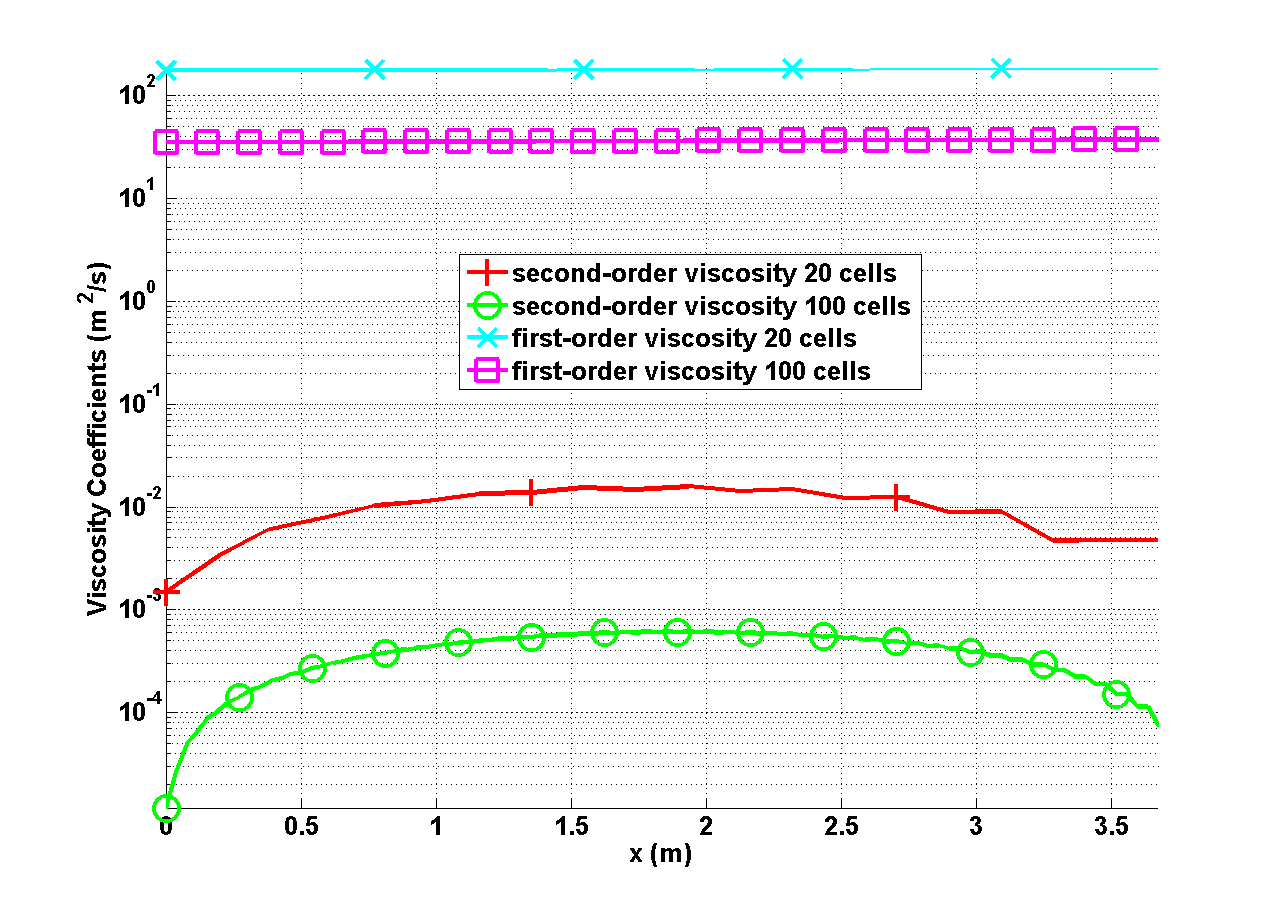
\includegraphics[scale=0.4]{plots/PWR_stt_viscosity.png}
\caption{PWR test case: axial viscosity profile}
\label{fig:Viscosity}
\end{figure}
In \fig{fig:Pressure}, the steady-state pressure profile obtained with the SUPG method shows a small non-physical change of slope at the outlet that does not disappear when a finer mesh is used. This artifact is not seen when using the entropy viscosity method. \\

It is noted from Figures~\ref{fig:Pressure} through~\ref{fig:Viscosity} that the first-order viscosity solution becomes ill-scaled. This is due to the low-Mach nature of the flow under consideration (flow speed around 5 m/s while the speed of sound is around 1,500 m/s). We carry out a low Mach limit study for the continuity equation written with its artificial dissipative term. The same reasoning can be applied as well to the momentum and energy equations. The first step consists of defining dimensionless variables, denoted by $(\tilde{\cdot})$ as follows:
\begin{equation}
\rho = \tilde{\rho} \rho^* \text{, } u = \tilde{u} u^* \text{, } x = \tilde{x} L \text{, } t = \tilde{t} \frac{u^*}{L} \text{ and } \kappa = \tilde{\kappa} \kappa^* 
\end{equation}
Using these definitions in the continuity equation yields
\begin{equation}
\label{eq:cont_proof}
\partial_{\tilde{t}} \tilde{\rho} + \tilde{\nabla} \cdot \left( \tilde{\rho} \vec{\tilde{u}} \right) =  \frac{k^*}{L u^*}  \tilde{\nabla}  \cdot  \left( \tilde{\kappa}  \tilde{\nabla} \tilde{\rho} \right).
\end{equation}
The coefficient $k^*$ depends upon whether the first- or entropy-order viscosity coefficient is employed. When using the first-order viscosity, \eqt{eq:equation15}, an expression for $\kappa^*$ is: $\kappa^* = \frac{L}{2}\left( \vec{u^*} + c^* \right)$. By substituting this definition into \eqt{eq:cont_proof}, the expression obtained for the scaled continuity equation is
\begin{equation}
\label{eq:cont_proof2}
\partial_{\tilde{t}} \tilde{\rho} + \tilde{\nabla} \cdot \left( \tilde{\rho} \vec{\tilde{u}} \right) = \frac{1}{2}\left( 1 + \frac{1}{M^*} \right)  \tilde{\nabla} \cdot \left(\tilde{\kappa}\tilde{\nabla} \tilde{\rho} \right),
\end{equation}
where $M^*$ is a reference Mach number. Thus, for low Mach flow the dissipative term will become ill-scaled and will alter the solution greatly
when using the first-order viscosity. However, when employing the entropy-viscosity coefficient \eqt{eq:ent_visc_coeff2} in the low Mach limit with 
$\tilde{P} = \rho^* (c^2)^* P$, the dissipative term is well-scaled:
\begin{equation}
\label{eq:cont_proof3}
\partial_{\tilde{t}} \tilde{\rho} + \tilde{\nabla} \cdot \left( \tilde{\rho} \vec{\tilde{u}} \right) =  \tilde{\nabla} \cdot  \left(\tilde{\kappa}\tilde{\nabla}  \tilde{\rho} \right).
\end{equation}
Obviously, it is therefore critical to evaluate, and if needed, to adapt the definition of the viscosity coefficients employed with the dissipative terms to a wide range of flow speeds.

A good way to assess the impact of the dissipative terms on the steady-state solution is to plot the mass flux (or momentum density) variable. It is expected to be constant in the low Mach limit, in the absence of a mass source and under the condition of having well-scaled dissipative terms, \eqt{eq:cont_proof2} and \eqt{eq:cont_proof3}.

\begin{figure}[h]
\centering
%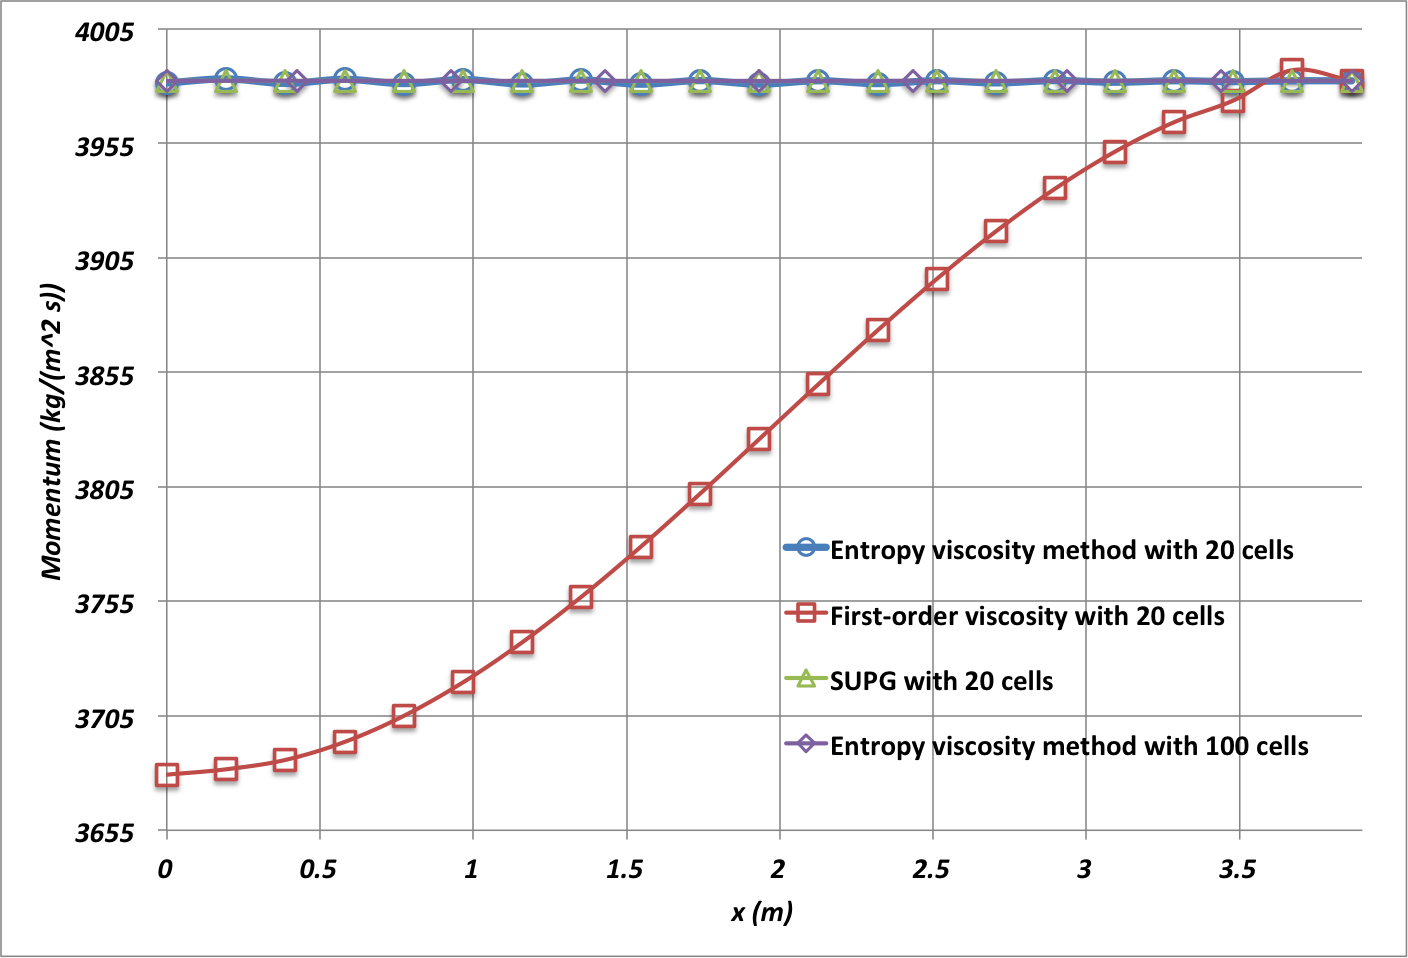
\includegraphics[scale=0.4]{plots/Momentum.png}
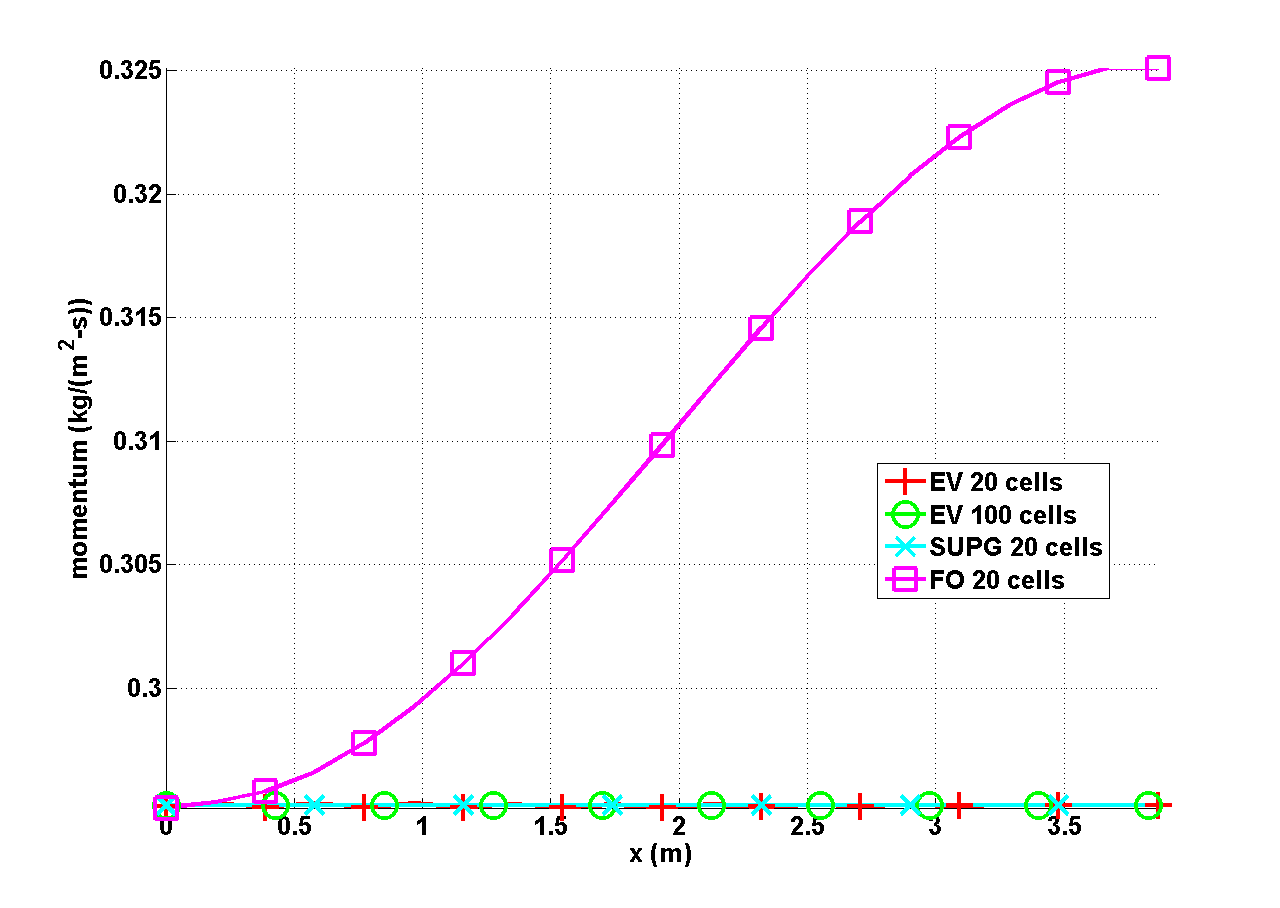
\includegraphics[scale=0.4]{plots/PWR_stt_momentum.png}
\caption{PWR test case: axial mass flux (or momentum) profile}
\label{fig:Momentum}
\end{figure}
This is shown in \fig{fig:Momentum}, where it is clear that the mass flux (or momentum density) remains constant ($0.2953$ $kg/(m^2.s)$) through the domain at steady-state when using either the entropy viscosity method or SUPG. When run with the first-order viscosity, the steady-state mass flux displays a $10\%$ variation over the domain because of the $\frac{1}{M^*}$ coefficient in the dissipative term of \eqt{eq:cont_proof2}.
%------------------------------------------------------------------------------
%
%------------------------------------------------------------------------------
\section{Conclusions} 
\label{sect::ccl}

We have extended the entropy viscosity method to fluid conservation equations (Euler equations) that contains terms pertaining to wall friction, gravity, and heat sources/sinks. This was achieved by enforcing that the entropy minimum principle be satisfied when the definition of the entropy residual was augmented to include the contribution of the heat source/sink terms.

The newly adapted technique has also been applied to a 1D pipe problem representative of a PWR channel under normal operating conditions. The artificial dissipative terms facilitate the correct physical solution when the higher-order viscosity coefficients are used. However, the solution obtained with the first-order viscosity is not correct.
Using the first-order viscosity definition resulted in that term being ill-scaled in the low-Mach limit. However, the entropy viscosity coefficient did not show such ill-scaling as Mach $\rightarrow 0$.

The steady-state solution is correctly resolved even with relatively coarse spatial nodalization using the continuous finite element approach implement in RELAP-7.

%------------------------------------------------------------------------------
%
%------------------------------------------------------------------------------
\section*{ACKNOWLEDGMENTS}

The authors would like to thank the RELAP-7 team from Idaho National Laboratory for providing RELAP-7 Code and the physical model used in this paper.

%------------------------------------------------------------------------------
% Bibliography. There are two ways to include the bibliography in your manu-
% script: 
% 1. use BibTeX: put physor2014.bst in your working directory  -or-
% 2. Manual list of references
% BibTeX is the preferred method, as it will take care of sorting etc automa-
% tically. To use BibTeX you need to make a database (.bib file), see the 
% example in the template. Many programs are available to make a BibTeX data-
% base for you, for example:
% - PyBliographer (http://www.pybliographer.org/)
% - Jabref        (http://jabref.sourceforge.net/)
%
% For BibTeX users: include as many bibliographic details as possible. The 
% physor2014.bst style file will select the relevant fields from your .bib file.
% Most bibliographic data are optional; if a required entry is missing BibTeX
% will complain about it.
% The physor2014.bst file allows the following non-standard options
% - a "doi" field, which will show as http://dx.doi.org/doi_number
% - a "url" field, which will set URLs in the proper way
% - the doi and url fields are processed by hyperref and result in clickable 
%   links
%
% In all cases (both for manual entry and for bibtex): 
% - The authors full name is preferred over initials (i.e. "Mercedes Benz" is 
%   preferred over "M. Benz")
% - List a maximum of three authors, separated by commas. If there are more than
%   threee authors, use "First Author \emph{et al},"
% - List as much bibliographic details as possible but if data are missing then
%   just leave the entries blank
%
% If you use BibTeX: 
%\bibliographystyle{physor2014}
%\bibliography{physor2014}

\begin{thebibliography}{11}

  \bibitem{relap7}
  \emph{RELAP-7 Theory Manual},
  R. A. Berry, et al., Idaho National Laboratory report, in preparation, 2014.
    
  \bibitem{Moose}
  \emph{A parallel computational framework for coupled systems of nonlinear equations},
  D. Gaston, C. Newsman, G. Hansen and D. Lebrun-Grandie, Nucl. Eng. Design, vol 239, pp 1768-1778, 2009.
  
  \bibitem{SUPG}
  \emph{Finite element formulations for convection dominated flows with particular emphasis on the compressible Euler equations},
  TE Tezduyar, TJR Hughes, Proceedings of the AIAA 21st Aerospace Sciences Meeting AIAA Paper 83-0125. Reno, Nevada, 1983.
  
  \bibitem{valentin}
  \emph{Implementation of the entropy viscosity method with the discontinuous Galerkin method},
  Valentin Zingan, Jean-Luc Guermond, Jim Morel, Bojan Popov, Volume 253, 1 January 2013, Pages 479-490
  
    \bibitem{jlg1}
  {\em Entropy viscosity method for nonlinear conservation laws}, 
  Jean-Luc Guermond, R. Pasquetti, B. Popov, J. Comput. Phys., 230 (2011) 4248-4267.
  
    \bibitem{jlg2}
  {\em Entropy Viscosity Method for High-Order Approximations of Conservation Laws}, 
  J-L. Guermond, R. Pasquetti, 
  Lecture Notes in Computational Science and Engineering, Springer, Volume 76, (2011) 411-418.
  
  \bibitem{jlg}
  \emph{Viscous regularization of the Euler equations and entropy principles},
  Jean-Luc Guermond and Bojan Popov, under review.
  
    \bibitem{Parabolic}
  \emph{On positivity preserving finite volume schemes for Euler equations},
  Perthane B. and Shu C-W., Numer. Math., 73(1):119-130, 1996.
  
  \bibitem{Relap7PWR}
  \emph{RELAP-7 level 2 milestone report: demonstration of a steady-state single phase PWR simulation with RELAP-7}
  D. Anders, R. Berry, D. Gaston, R. Martineau, J. Peterson, H. Zhang, H. Zhao, L. Zou, Idaho National Laboratory report INL/EXT-12-25924, May 2012.
  
  \bibitem{SGEOS}
  \emph{Elaborating equation of state for a liquid and its vapor for two-phase flow models.}
  O. LeMetayer, J. Massoni, R. Saurel, International Journal of Thermal Science 43 (2004) 265-276.

\bibitem{Toro}
  \emph{Riemann Solvers and numerical methods for fluid dynamics.}
  E.F. Toro, $2^{nd}$ Edition, Springer.  
  
  %\bibitem{LowMach}
    %\emph{Preconditioned techniques in computational fluid dynamics.}
  %E.Turkel, Annu. Rev. Fluid Mech. (1999) 31:385-416.  
  
%\bibitem{SEM}
  %\emph{The discrete equation method (DEM) for fully compressible, two-phase flows in ducts of spatially varying cross-section.}
  %R. Berry, R. Saurel, O. LeMetayer,
  %Nuclear Engineering and Design, 240 (2010) 3797-3818.
  \end{thebibliography}

%
% If you use manual input, use the following format.
%------------------------------------------------------------------------------
% \begin{thebibliography}{300}
% \bibitem{journal} Some Author(s), ``Article Title,'' \emph{Journal Name}, \textbf{Volume(number)}: pp. 34-89 URL \url{http://dx.doi.org/doi_number} (19xx).
%
% \bibitem{proc_paper} C. D. Author(s), ``Article Title,'' In: \emph{Proceedings of Meeting} (Editor Name, editor), Organisation, Location, Dates of Meeting, Vol. n: pp. 134-156 (19xx).
%
% \bibitem{book} Epsilon F. Author, \emph{Book Title in Italic}, Publisher, City \& Country (19xx). 
%
% \bibitem{website} ``Research Institute of Nuclear Engineering, University of Fukui'', \url{http://www.rine.u-fukui.ac.jp/english/index.html} (2013).
% \end{thebibliography}
%
%------------------------------------------------------------------------------
% Set up for appendices
%------------------------------------------------------------------------------
%\appendix
%
%\makeatletter
%\def\@seccntformat#1{APPENDIX \csname the#1\endcsname.~}
%\makeatother

%------------------------------------------------------------------------------
% If you need to make one (or more) appendix (appendices), place them here as
% sections
%------------------------------------------------------------------------------
%\section{HOW TO MAKE APPENDICES}
%\label{app::a}
%
%An appendix is a section with extra material which is relevant to the manuscript, but is too bulky, too detailed, or simply too long to include in the main text. Feel free to make one (or more) appendix (appendices), but remember: if you make an appendix, then you must include a reference from the main text to the appendix. An unreferenced (``dangling") appendix is not allowed.
%
%\section{ISSUES RELATED TO FISSION PRODUCT DECOUPLING IN ADJOINT TRANSMUTATION CALCULATIONS}
%\label{app::b}
%
%An appendix is a section with extra material which is relevant to the manuscript, but is too bulky, too detailed, or simply too long to include in the main text. Feel free to make one (or more) appendix (appendices), but remember: if you make an appendix, then you must include a reference from the main text to the appendix. An unreferenced (``dangling") appendix is not allowed.

\end{document}

%------------------------------------------------------------------------------
% pdflatex allows figures in PDF, JPG and PNG. For users who have prepared their
% figures in (e)ps, please find here some tips and tricks:
% - Nearly all latex distributions have the tool "ps2pdf". This tool translates 
%   (e)ps files into pdf files, which can be included in pdflatex
% - In some cases, ps2pdf produces a pdf file on a4 size (or US letter size, de-
%   pending on your computer's settings). In such a case, use "pdfcrop" to cut 
%   off the excess white space. Subsequently include the cropped pdf file (by
%   default the file foo.pdf will be renamed foo-crop.pdf). Note: do NOT use
%   foo.crop.pdf! pdflatex will complain that .crop.pdf is not a known graphics
%   format.
% - If you have very many (e)ps files that need conversion, consider making a 
%   BASH script or something similar and use ps2pdf and pdfcrop on each (e)ps
%   file
%------------------------------------------------------------------------------

